\section{PCB Design Errors}
No project would be complete without something going wrong. Our project was no exception. Both during PCB design and after receiving our manufactured PCB, we started to discover various complications. This section discusses the more serious ones in detail, and what we did to solve the problem.

\subsection{Routing Problems}
\label{Routing Problems}
As mentioned earlier, we encountered several complications during the routing procedure. Most of them were a product of bad Altium settings, and they took some time to find, since we were quite inexperienced with Altium.
The most significant ones are described in detail in the following sections.

\subsubsection{Bad Auto Router Settings}
After auto routing the whole thing the first time, the result was disappointing. It contained over 100 still unrouted connections, which means the auto router didn't manage to connect these.
\newline
\newline
We discovered that choosing different routing options for the auto router made a big difference. The default setting was \emph{Default 2 Layer Board}. Hence, the auto router focused on mainly using the top and bottom layer, and avoiding layer-switching. This resulted in the auto router not being able to route all the necessary connections.
\newline
\newline
After making the auto-router focus more on switching layers for every signals, to avoid complex routing on fewer layers, it managed to route all the connections. This was achieved by changing routing strategy from \emph{Default 2 Layer Board} to \emph{Default Multi Layer Board} in Altium.

\subsubsection{Clearance Constraint Issue}
After the first auto routing attempts, we got tons of short-circuits. We found out that our clearance constraint rule didn't apply for all components. The reason for this was a HDMI rule we had self-defined. The pads on the HDMI were placed so close together that we had to lower the clearance constraint for this component. To bypass this, we removed the general clearance constraint rule and instead made a new one to count for all traces, except for HDMI ones. This turned out to be a huge mistake, because now Altium couldn't find this general clearance constraint. This mistake lead to Altium not caring at all about clearances, thus routing as it pleased, which resulted in a short-circuit nightmare.
\newline
\newline
Adding the general clearance constraint rule back again, we faced the same issue in another form. The auto router wouldn't route at all, because it complained about clearance constraints violations.
\newline
The clearance constraint rule was still the issue. The settings said that Altium would check for clearance violation with \emph{Any Net}. Thanks to some help from Odd Rune, we discovered that \emph{Any Net} also included the net that it was currently comparing. Thus, it checked if the current trace meets the clearance constraint with itself, which of course it does not. By changing this setting to \emph{Different Nets Only}, the entire short-circuit problem was solved. 

\subsubsection{Dead Copper}
Dead copper is parts of the copper on a power plane that's isolated from the rest of the copper on that plane. 
Dead copper appeared several places on our PCB. Normally it wasn't a problem, but some places a GND via or 3.3V via was connected to dead copper on the corresponding power plane. This had to be fixed, since this via would have no contact with the rest of the plane.
\newline
We had to avoid power vias connected to dead copper, so we located every position where this situation occurred, and repositioned neighboring vias to rejoin the copper area with the rest of the copper plane. The issue and solution are described in figure \ref{fig:Dead copper}.

\begin{figure}[h!]
\centering
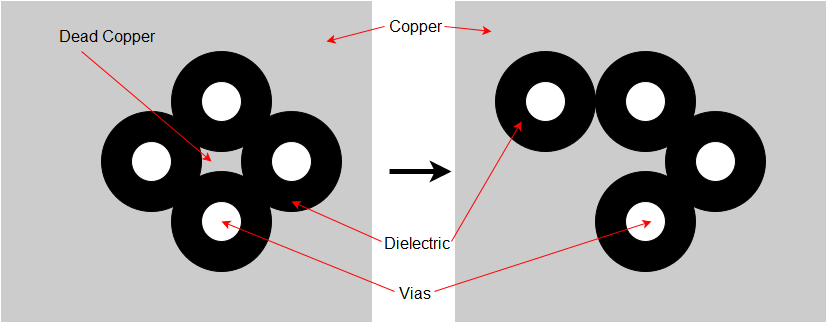
\includegraphics[scale = 0.4]{images/Dead_Copper.png}
\caption{Dead Copper. To the right, dead copper is avoided by moving one via}
\label{fig:Dead copper}
\end{figure}

\subsection{Possible Routing Improvement}
Since the auto router did the biggest part of the job, some wires took long detours, because of the complexity. Manual routing of some signals could've shortened these distance. However, the distance from a point to another wasn't critical for our design, since the signals travel very fast and we didn't have to keep a strict time schedule. Therefore, we decided it wasn't worth the time.

Wires in the same parallell bus, should ideally have equal lengths, to make sure all signals in the same bus were synchronized. Some of our wires in the EBI bus and the bus between the FPGA and the frame buffer, had varying lengths. Again, the time differences would be so small that they wouldn't have a noticable effect on our design, but for a high-speed modern computer, it is critical to avoid these race conditions \cite{race-conditions}.

\subsection{Bad Soldering}
Some issues arised because of components not being properly soldered onto the PCB. Examples could be component pins having partial or no contact with the PCB, or pins touching several pads, when pads were tightly arranged.

\subsubsection{Partially Soldered Voltage Regulator} 
It was very important to verify that the power planes worked as we intended. Obviously, nothing would work without power. Hence, this was the very first test we performed.
\newline
Everything necessary for power to be present, was soldered on. This included power headers, and the 3.3 voltage regulator. External power was inserted through power headers. By measuring different places with a multimeter, we already discovered anomalies. The voltmeter showed only 2.3V instead of 3.3V. Further testing revealed that one of the voltage regulator pins hadn't been soldered properly, resulting in a loss of 1V. After fixing this, the digital VCC plane contained the correct 3.3V.

\subsection{Incorrect Wiring}
Most PCB problems were due to incorrect wiring. Either signals were having unexpected values, short-circuits had occurred, or other unexpected behaviour. In the next sections, the most significant wiring issues are addressed and how they were fixed.

\subsubsection{Short-circuits in Buttons}
We discovered that our buttons were wired wrong, since they caused short-circuits. The reason was sloppy study of the datasheet, as shown in figure \ref{fig:Button Issue}. Luckily, this could be remedied by rotating the button 90 degrees, if we adjusted the physical connectors to fit the footprint.

\begin{figure}[h!]
\centering
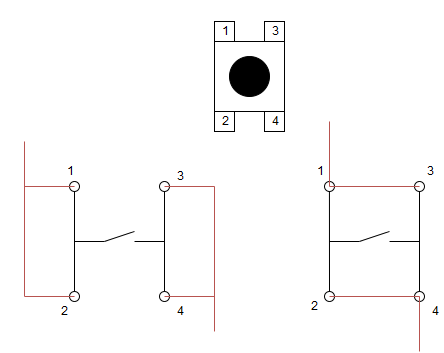
\includegraphics[scale=0.5]{images/Button_Issue.png}
\caption{Top figure shows the button as it looks like on the PCB. On the left: Correct wiring according to datasheet. On the right: Incorrect wiring leading to short-circuit}
\label{fig:Button Issue}
\end{figure}

\subsubsection{No Output from Oscillators}
When testing the oscillators, they did not seem to work. The datasheet for these components clearly stated that connecting the E/D pin to either 'No Connect' or '1' equaled active, so we did not connect it. We tried to remedy by connecting E/D to Vcc, and the problem was solved.

\subsubsection{Incorrect Power Supply to Vref and DACs}
The Vref chip was supplied with 3.3V, but should have been supplied with analogue 5V instead. This could be remedied by cutting on the 3.3V power trace, since the trace is located on the top layer and no other traces are beneath it. Then we could connect analogue 5V via header from the voltage regulator to the input pin on the Vref chip.
\newline
The DACs were supplied with analogue 5V, but should have been supplied with 3.3V. The analogue 5V should go to the Vref chip instead. This was solved by switching the two connections.

\subsubsection{Faulty Connected BNCs}
The BNC connections were faulty wired. Each BNC had two connections excluding the socket itself connected to the BNC cable. One of these would go to ground, while the other would receive the signal destined for the oscilloscope. The PCB was incorrectly wired, leading to these connections being switched. This lead to a negative voltage output to the oscilloscope, which resulted in an inverted image. 

\subsubsection{FPGA Configuration Issue}
When the FPGA would complete configuration it was supposed to set a signal high, which was connected to the MCU, saying it was ready. However, the MCU seemed to ignore this signal, because it never changed. What caused this problem was too hasty study of the manual describing configuration of the FPGA.
An unnecessary connection to VCC, forced the Done signal into the MCU to always be high, even when the FPGA was not configured. We couldn't remove the VCC connection, so we had to figure out a workaround.

By introducing a transistor, and making the signal active low on the MCU side, we managed to make the MCU notice when configuration was complete.
The problem and solution is shown in detail in figure \ref{fig:Done Issue}.
This solution was possible because the wire went through the JTAG header. 

\begin{figure}[h!]
\centering
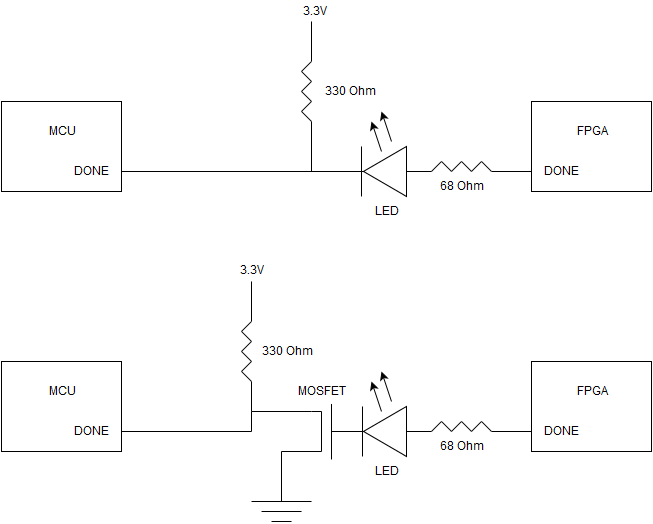
\includegraphics[scale=0.5]{images/Done_Signal_Issue.png}
\caption{Problem and solution of Done signal
         \newline
         Top: Done signal into MCU was always logical high
         \newline
         Bottom: Done signal into MCU was now active low. The transistor was activated when the configuration was complete, forcing the 3.3V to ground}
\label{fig:Done Issue}
\end{figure}

After further studying of the FPGA configuration manual, we saw that this guide was different from what we intended in our design, so there was need for this extra VCC connection. The guide we studied is on page 42 in \cite{fpga-configuration}

\subsubsection{Noise Reduction}
The diode which we intended to reduce noise in the analogue plane, had no noticable effect. The reason was probably that we only thought about current leakage and not noise itself. To solve this problem, the team got the idea of using a ferrite bead instead of the diode. A ferrite bead is a component designed to suppress high-frequency noise. 
\newline
Noise was reduced, but the ferrite bead itself worked also as a resistor, allowing only a small current flow through. By connecting a resistor with very low resistance (How many Ohms?) in parallell with the ferrite bead, current was able to flow freely through this connection.